\documentclass[../portafolio.tex]{subfiles}



\begin{document}

\section{Ecuaciones diferenciales ordinarias} 

\hfill \textbf{Fecha de la actividad:} 23 de septiembre de 2022

\medskip


%---------------------------------------------------------------------------------
\subsection{Objetivo de la clase}
En este laboratorio se aprendió a usar el método de Euler-Cromer para resolver ecuaciones diferenciales ordinarias, específicamente se trabajó con las ecuaciones \ref{LVec1} y \ref{LVec2} de Lotka-Volterra. Estas son un par de ecuaciones diferenciales de primer orden no lineales que se usan para describir dinámicas de sistemas biológicos en el que dos especies interactúan, una como presa y otra como depredador\cite{lotkavolterra}.




\begin{align}
    \frac{dP}{dt} &=\alpha P-\beta PD  \label{LVec1}\\
    \frac{dD}{dt} &= -\gamma D +\delta PD \label{LVec2}.
\end{align}

En este laboratorio trabajé junto a Mauricio Bastías.

\subsection{Desarrollo del laboratorio}

Las ecuaciones \ref{LVec1} y \ref{LVec2} de Lotka-Volterra se pudieron reducir a las ecuaciones \ref{LVec3} y \ref{LVec4} que dependen de una solo constante $\mu$. 

\begin{align}
    \frac{d\Pi}{d\tau} &= \Pi (1-\Delta) \label{LVec3} \\
    \frac{d\Delta}{d\tau} &= \mu \Delta(\Pi -1) \label{LVec4}.
\end{align}

Para ello se definió $t =\tau / \alpha$, $ P = \Pi \gamma / \delta $ y $D = \alpha \Delta / \beta$. Luego, reemplazando estos valores en \ref{LVec1}:

\begin{align*}
    \frac{d\frac{\Pi\gamma}{\delta}}{d\frac{\tau}{\alpha}} &= \alpha \left( \frac{\Pi \gamma}{\delta} \right) - \beta \left( \frac{\Pi \gamma}{\delta} \right) \left(  \frac{\alpha \Delta}{\beta}      \right) \\
    \frac{d\Pi}{d\tau}\left( \frac{\alpha \gamma}{\delta} \right) &= \alpha \left( \frac{\Pi \gamma}{\delta} \right) -  \left( \frac{\Pi \gamma}{\delta} \right)  \alpha \Delta \\
    \frac{d\Pi}{d\tau} &= \Pi - \Pi \Delta \\
    \frac{d\Pi}{d\tau} &= \Pi (1-\Delta)
\end{align*}
 
 Ahora reemplazando en la ecuación \ref{LVec2} se tiene:
 
 \begin{align*}
     \frac{d\frac{\alpha \Delta}{\beta}}{d\frac{\tau}{\alpha}} &=  -\gamma \left(\frac{\alpha \Delta}{\beta} \right)  +  \delta \left(\frac{\Pi \gamma}{\delta}\right) \left(\frac{\alpha\Delta}{\beta}\right) \\
     \frac{d\Delta}{d\tau} \left( \frac{\alpha^2}{\beta}\right) &=     -\gamma \left(\frac{\alpha \Delta}{\beta} \right)  +  \Pi \gamma \left(\frac{\alpha\Delta}{\beta}\right)\\
     \frac{d\Delta}{d\tau} &= -\frac{\gamma}{\alpha} \Delta  + \frac{\gamma}{\alpha} \Pi \Delta\\
\end{align*}

Finalmente, definiendo $\mu= \frac{\gamma}{\alpha}$ queda:

\begin{equation}
     \frac{d\Delta}{d\tau} = \mu\Delta\left( \Pi - 1\right)
\end{equation}

\vspace{5mm}
Para resolver estas ecuaciones diferenciales ordinarias se creó el código \ref{c1LV}  con una función \texttt{LV} con variables \texttt{P0, V0, mu, tmax} y \texttt{h} donde las primeras dos variables correspondían a $\Pi(0)$ y a $\Delta(0)$, respectivamente, \texttt{tmax} corresponde al tiempo máximo, \texttt{mu} al valor de la constante $\mu$ y \texttt{h} el paso del tiempo. 

\begin{listing}[h]
    \begin{minted}[
frame=lines,
framesep=2mm,
baselinestretch=1.2,
bgcolor=LightGray,
fontsize=\footnotesize,
linenos
]
{python}
def Lotka_Volterra(P0,D0,mu,tmax,h):
    t= np.arange(0,tmax,h)
    P= np.zeros(len(t))
    D= np.zeros(len(t))
    P[0]=P0
    D[0]=D0
    for n in range(len(t) - 1):
        P[n+1]= P[n] + h * P[n] * (1- D[n])
        D[n+1]= D[n] + h * mu * D[n] * (P[n+1] - 1)
    return t, P, D
    \end{minted}

\caption{Función que resuelva le ecuación diferencial ordinaria de Lotka-Volterra a través del método de Euler-Cromer}
\label{c1LV}
\end{listing}

En la tercera y cuarta linea del código \ref{c1LV} se definió \texttt{P} y \texttt{D} como un \texttt{arange} de ceros de un número de dimensiones igual al número de valores que tiene \texttt{t}, luego en las siguientes dos lineas se define el primer valor de los \texttt{arange} de \texttt{P} y \texttt{D}. Finalmente de la línea 7 se ejecuta un ciclo \texttt{for} que resuelve la ecuación diferencial ordinaria de Lotka-Volterra retornando los valores de \texttt{t, P} y \texttt{D}. Además, en la línea 9 se hace el cálculo con \texttt{P[n+1]}, debido a que este ya fue calculado en la línea anterior.

\vspace{5mm}
Luego, se evaluó la función \texttt{LV} para $tmax=40$, $P0=1$, $V0=5$, $\mu=1$ y $h=0.001$ obteniendo así los valores de $D$ y $P$. Luego estos se graficaron en función del tiempo resultando el gráfico \ref{graf1LV}
\vspace{5mm}


\begin{figure}
    \centering
    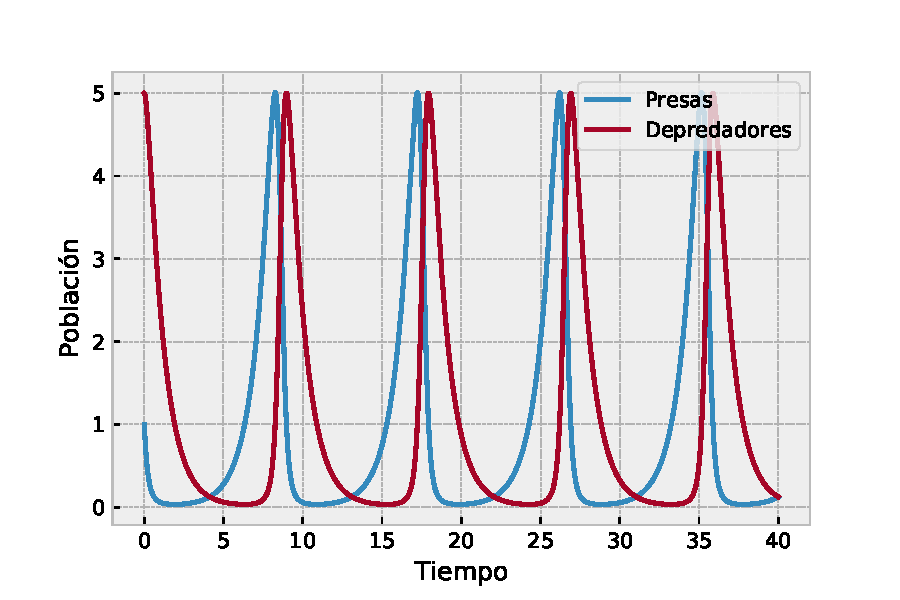
\includegraphics[scale=0.85]{tex/img/edo-ej-c.pdf}
    \caption{Gráfico de la población de presas y depredadores en el modelo de Lotka-Volterra con la constante $\mu=1$.}
    \label{graf1LV}
\end{figure}

Del gráfico \ref{graf1LV} se pudo interpretar que cuando el número de presas es mínimo el número de depredadores poco tiempo después comienza a decaer, pues estos se encuentran sin alimento, luego con la disminución de depredadores más adelante el número de presas vuelve a aumentar hasta llegar a su máximo y el proceso se vuelve a repetir cíclicamente.

\vspace{5mm}
Se resolvió la ecuación diferencial de Lotka-Volterra pero ahora con $tmax=0$ y con $\Delta(0)$ variando entre $1,1$ y $10$. Para ello se creó un ciclo \texttt{for} donde \texttt{V0} tomaba 20 valores distintos y para cada valor que tomaba \texttt{V0} se graficaba una curva, obteniéndose así el gráfico \ref{graf2LV}. De este gráfico se puede deducir que mientras mayor sea la cantidad inicial de depredadores la caída del número de presas va a ser más brusco al igual que el aumento de depredadores.

\vspace{2mm}
Las ecuaciones de Lotka-Volterra admiten una forma constante que se puede apreciar en la ecuación \ref{cteLV}.


\begin{equation}
    C=\ln{\Delta}-\Delta + \mu (\ln{\Pi}-\Pi). \label{cteLV}
\end{equation}

El gráfico \ref{graf3LV} muestra a $C$ en función del tiempo para todos los valores que tomó $\Delta(0)$ en el gráfico \ref{graf2LV}. Además, La curvas son aproximadamente constante por lo tanto se puede decir que el método numérico desarrollado entrega soluciones aproximadamente tolerables a las ecuaciones diferenciales.

\begin{figure}
    \centering
    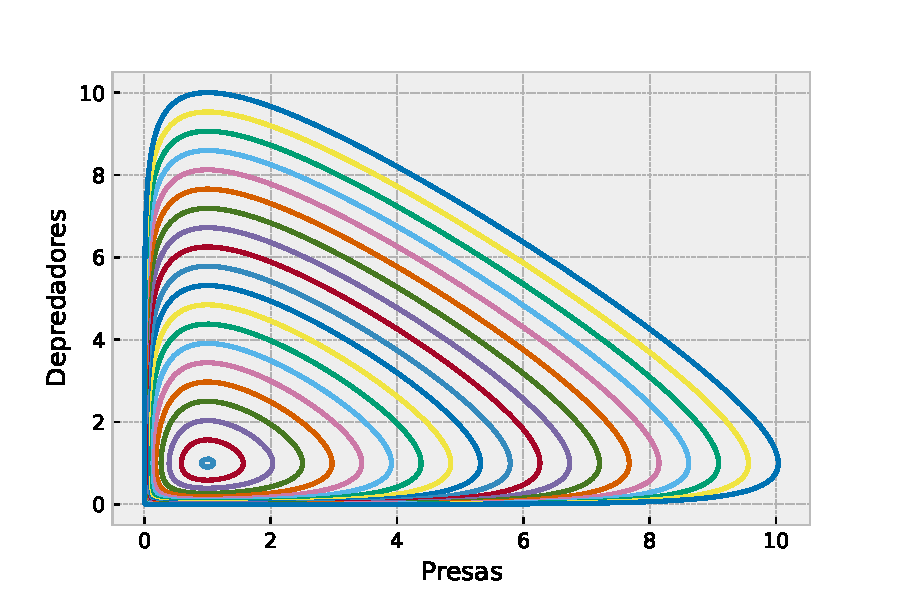
\includegraphics[scale=0.85]{tex/img/edo-ej-d.pdf}
    \caption{Espacio de fases del modelo de Lotka-Volterra}
    \label{graf2LV}
\end{figure}




\begin{figure}
    \centering
    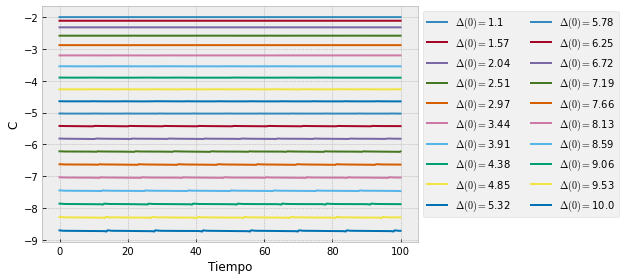
\includegraphics[scale=0.8]{tex/img/edo-ej-e.png}
    \caption{$C$ en función del tiempo para valores de $1.1<\Delta(0)<10$ usando $h=0.001$, donde mientras mayor es $\Delta(0)$ la curva se hace mas negativa.}
    \label{graf3LV}
\end{figure}






\subsection{Conclusiones}

En este laboratorio se partió reduciendo las ecuaciones de Lotka-Volterra para que dependieran de una sola constante $\mu$, luego se resolvieron estas ecuaciones diferenciales mediante con el método de Euler-Cromer. Seguidamente se estudió el número de la población de los depredadores y de las presas y como variaban en función del tiempo. Luego se graficó $\Delta(t)$ versus $\Pi(t)$  observando su relacionaban y como variaba la curva del gráfico según el valor inicial de los depredadores. Finalmente se graficó $C$ en función del tiempo concluyendo que el método numérico entregaba soluciones aproximadas tolerables.

\vspace{2mm}
Al desarrollar esta actividad aprendí que para resolver ecuaciones diferenciales ordinarias a través del método de Euler-Cromer son necesarios los valores iniciales y que si se tienen ecuaciones de orden mayor, entonces se pueden simplificar en un sistema de ecuaciones diferenciales ordinarias de primer orden con el fin de poder utilizar este método. Lo que no entendí muy bien fue la demostración del método y en cómo se programó el método.

\vspace{2mm}
Me hubiera gustado que se hubiera dispuesto un poco más de tiempo en cómo se programó el método, quizás desarrollando algún ejemplo simple utilizándolo antes de comenzar a desarrollar el laboratorio.




\end{document}